In this Section, the multiclass kernel perceptron algorithm presented in the theory part above is trained on the training set $S$ of the MNIST dataset for several settings. The multiclass predictors are trained using the three different realizations of the multiclass kernel perceptron algorithm. The performance of the trained multiclass predictors is evaluated on the test set $D$. The test error rates of the three realizations of the multiclass kernel perceptron algortihm are compared for different choices of the degree of the polynomial kernel $p$. In the present work, degrees from $p=1$ up to $p=6$ are applied. Each predictor is trained for a total of $N_{epoch}=10$ cycles over random permutations of the training examples in the training set $S$. The final result are three multiclass predictors - one for each realization of the multiclass kernel perceptron algorithm - that minimize the test error rate on the test set $D$, and that are compared with results on the classification of handwritten digits in the MNIST dataset in the literature in the next Section.

\subsection{Binary Predictors}\label{subsec:bin_pred}
Before presenting the obtained multiclass predictors, it is instructive to take a look at what happens at the heart of the multiclass kernel perceptron algorithm when performing a training on the training set $S$. As explained in the theory part, the multiclass kernel perceptron algorithm is a simple combination of ten binary predictors - one for each digit $a$. Here, exemplarily, the binary predictor $h_{S^{(5)}}$ for the digit $a=5$ is considered. Nonetheless, the key statements in this Subsection are valid for all of the ten digits. \\

Figure~\ref{fig:train_error_bin} shows the binary training error rates $\hat{\ell}_{S^{(5)}}$ as a function of the number of epochs $N_{epoch}$ for the six different degrees $p$ of the polynomial kernel. In each panel, the binary training errors for the final, the minimizing, and the average predictor are displayed. 

\begin{figure}[h!]
    \begin{subfigure}[t]{0.49\textwidth}
        \centering
        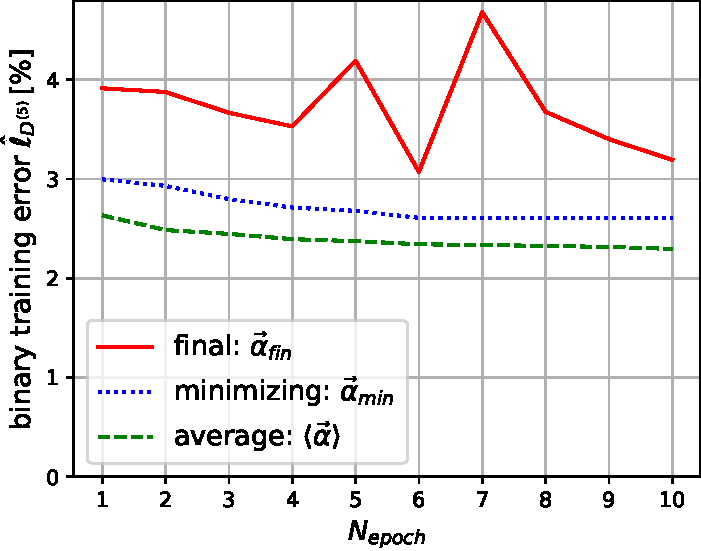
\includegraphics[width=\linewidth]{bin_pred/training_digit=5_deg=1.pdf} 
        \caption{$p = 1$}
    \end{subfigure}
    \hfill
    \begin{subfigure}[t]{0.49\textwidth}
        \centering
        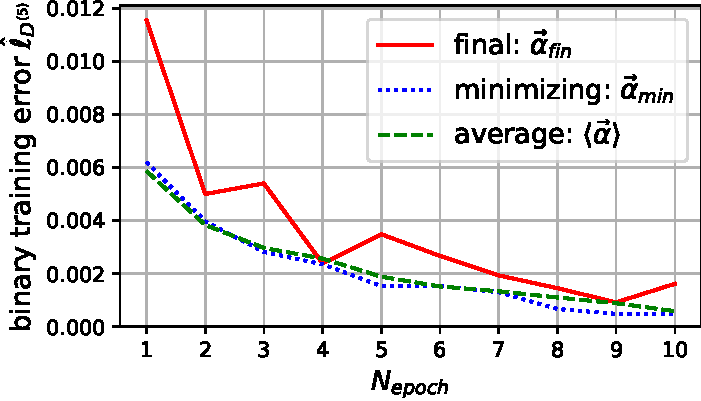
\includegraphics[width=\linewidth]{bin_pred/training_digit=5_deg=2.pdf} 
        \caption{$p = 2$}
    \end{subfigure}
    \par\bigskip
        \begin{subfigure}[t]{0.49\textwidth}
        \centering
        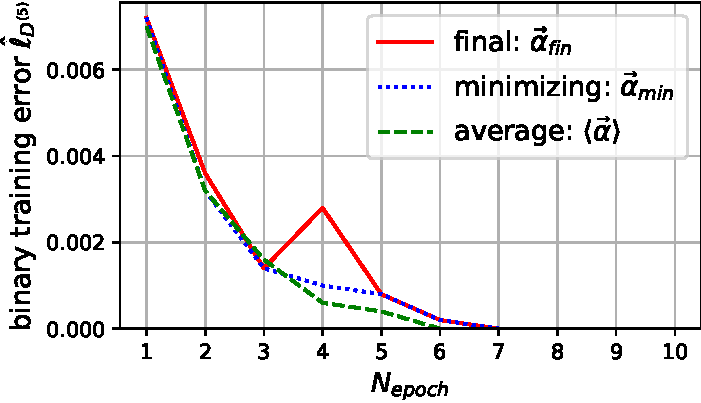
\includegraphics[width=\linewidth]{bin_pred/training_digit=5_deg=3.pdf} 
        \caption{$p = 3$}
    \end{subfigure}
    \hfill
    \begin{subfigure}[t]{0.49\textwidth}
        \centering
        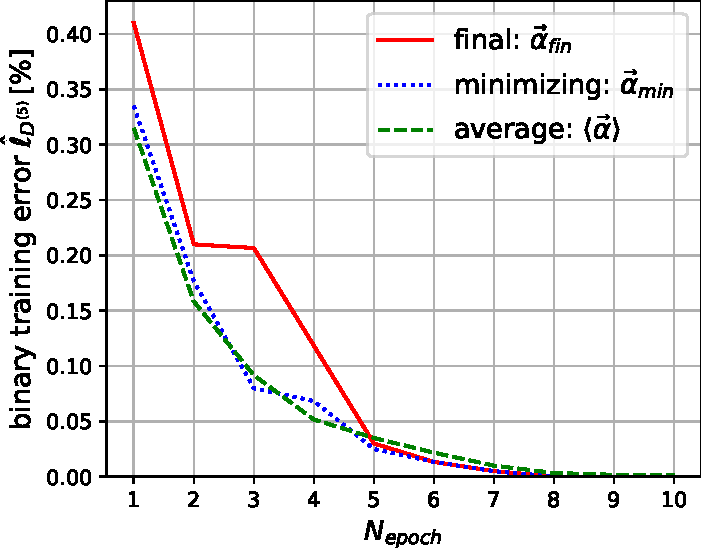
\includegraphics[width=\linewidth]{bin_pred/training_digit=5_deg=4.pdf} 
        \caption{$p = 4$}
    \end{subfigure}
    \par\bigskip
        \begin{subfigure}[t]{0.49\textwidth}
        \centering
        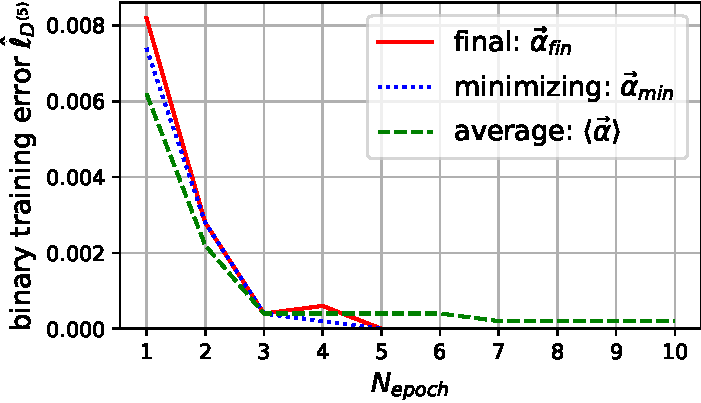
\includegraphics[width=\linewidth]{bin_pred/training_digit=5_deg=5.pdf} 
        \caption{$p = 5$}
    \end{subfigure}
    \hfill
    \begin{subfigure}[t]{0.49\textwidth}
        \centering
        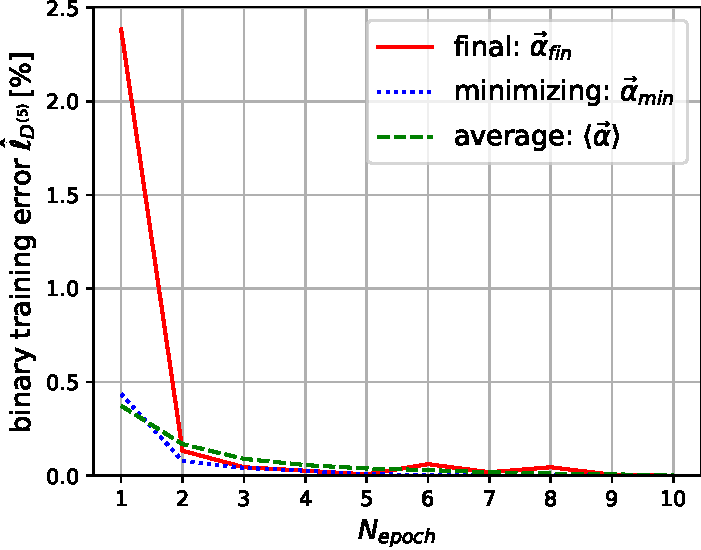
\includegraphics[width=\linewidth]{bin_pred/training_digit=5_deg=6.pdf} 
        \caption{$p = 6$}
    \end{subfigure}
    \caption{Binary training error rates $\hat{\ell}_{S^{(5)}}$ as a function of the number of epochs $N_{epoch}$ for the training of binary predictors that classify, whether an image shows the digit $a=5$ or not. Each panel displays the binary training error rates $\hat{\ell}_{S^{(5)}}$ for a different degree $p$ of the polynomial kernel for the three approaches to retrieve binary predictors from the binary kernel perceptron algorithm. Note, the different scales of the vertical axes. The binary test error rates for the same binary predictors are displayed in Fig~\ref{fig:test_error_bin}.}\label{fig:train_error_bin}
\end{figure}

\begin{figure}[h!]
    \begin{subfigure}[t]{0.49\textwidth}
        \centering
        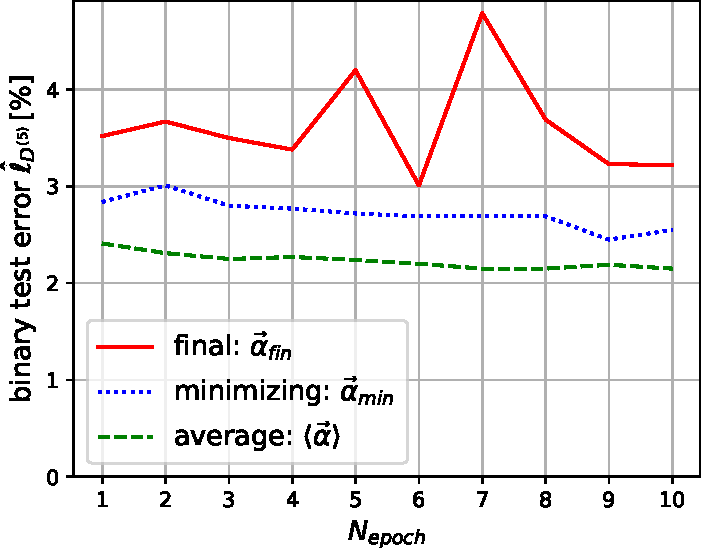
\includegraphics[width=\linewidth]{bin_pred/test_digit=5_deg=1.pdf} 
        \caption{$p = 1$}
    \end{subfigure}
    \hfill
    \begin{subfigure}[t]{0.49\textwidth}
        \centering
        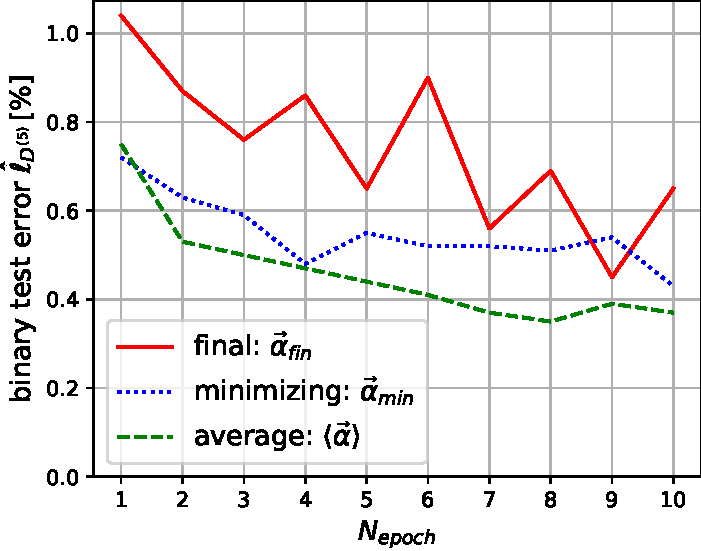
\includegraphics[width=\linewidth]{bin_pred/test_digit=5_deg=2.pdf} 
        \caption{$p = 2$}
    \end{subfigure}
    \par\bigskip
        \begin{subfigure}[t]{0.49\textwidth}
        \centering
        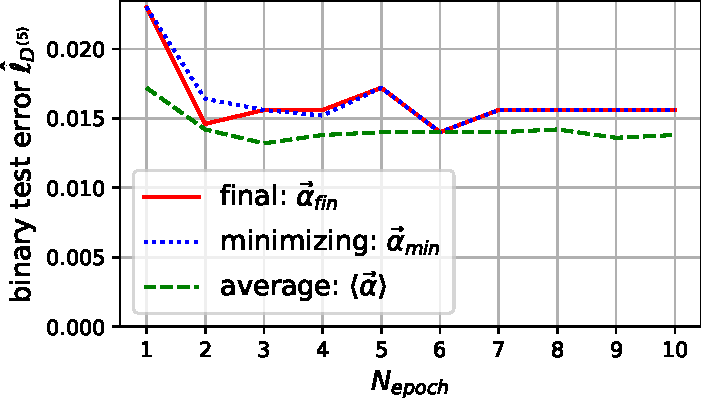
\includegraphics[width=\linewidth]{bin_pred/test_digit=5_deg=3.pdf} 
        \caption{$p = 3$}
    \end{subfigure}
    \hfill
    \begin{subfigure}[t]{0.49\textwidth}
        \centering
        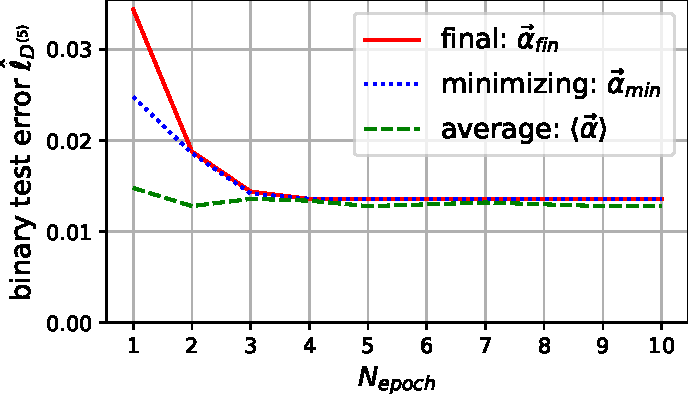
\includegraphics[width=\linewidth]{bin_pred/test_digit=5_deg=4.pdf} 
        \caption{$p = 4$}
    \end{subfigure}
    \par\bigskip
        \begin{subfigure}[t]{0.49\textwidth}
        \centering
        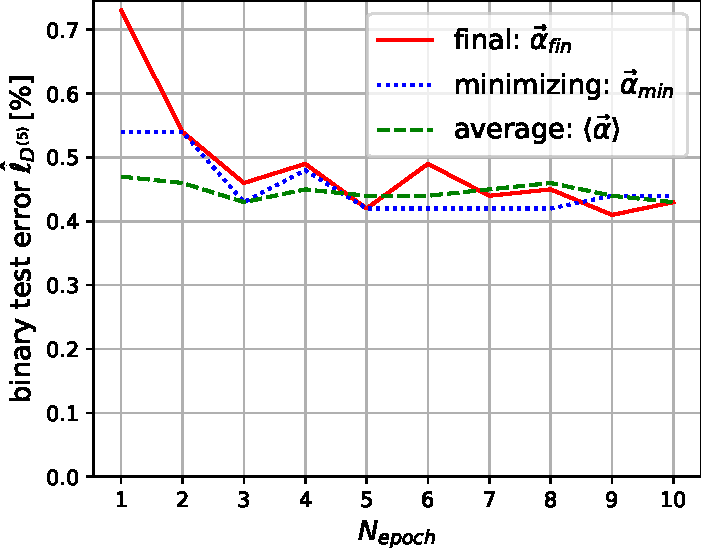
\includegraphics[width=\linewidth]{bin_pred/test_digit=5_deg=5.pdf} 
        \caption{$p = 5$}
    \end{subfigure}
    \hfill
    \begin{subfigure}[t]{0.49\textwidth}
        \centering
        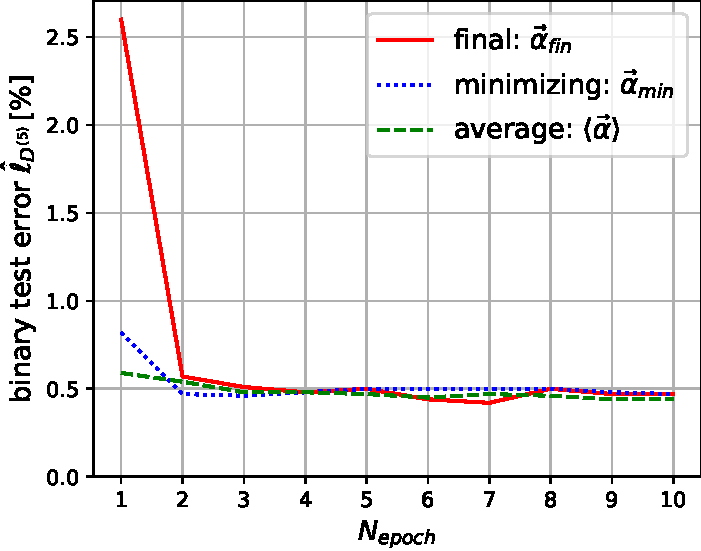
\includegraphics[width=\linewidth]{bin_pred/test_digit=5_deg=6.pdf} 
        \caption{$p = 6$}
    \end{subfigure}
    \caption{Binary test error rates $\hat{\ell}_{D^{(5)}}$ as a function of the number of epochs $N_{epoch}$ for the training of binary predictors that classify, whether an image shows the digit $a=5$ or not. Each panel displays the binary test error rates $\hat{\ell}_{D^{(5)}}$ for a different degree $p$ of the polynomial kernel for the three approaches to retrieve binary predictors from the binary kernel perceptron algorithm. Note, the different scales of the vertical axes. The binary training error rates for the same binary predictors are displayed in Fig~\ref{fig:train_error_bin}.} \label{fig:test_error_bin}
\end{figure}

\clearpage

\subsection{Multiclass Predictors}\label{subsec:multi_pred}

\begin{figure}[h!]
    \begin{subfigure}[t]{0.49\textwidth}
        \centering
        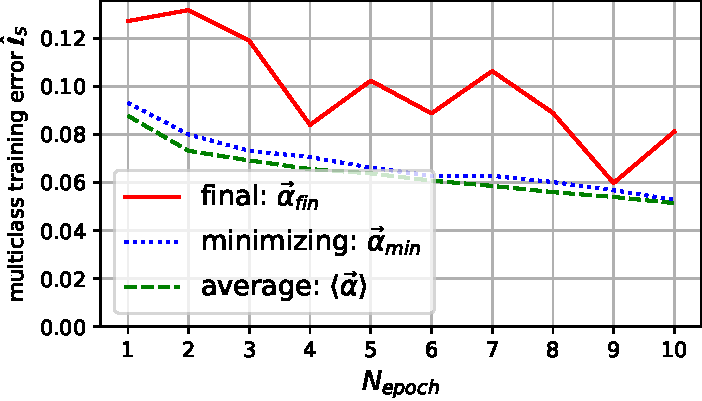
\includegraphics[width=\linewidth]{performance/training_deg=1.pdf} 
        \caption{$p = 1$}
    \end{subfigure}
    \hfill
    \begin{subfigure}[t]{0.49\textwidth}
        \centering
        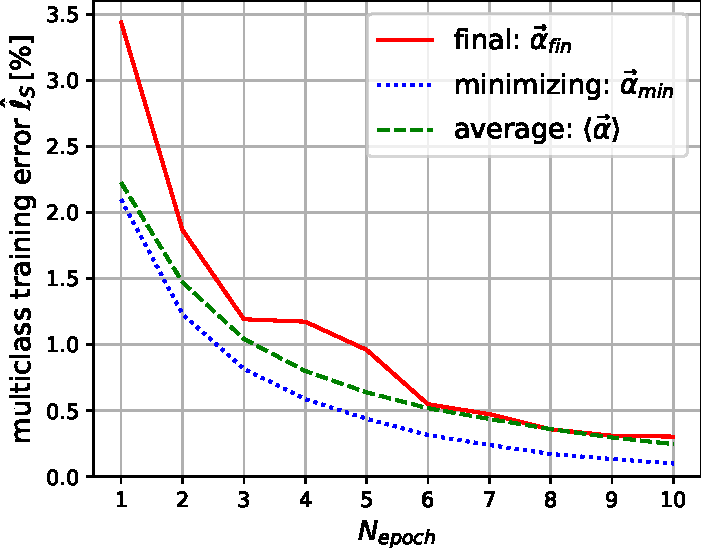
\includegraphics[width=\linewidth]{performance/training_deg=2.pdf} 
        \caption{$p = 2$}
    \end{subfigure}
    \par\bigskip
        \begin{subfigure}[t]{0.49\textwidth}
        \centering
        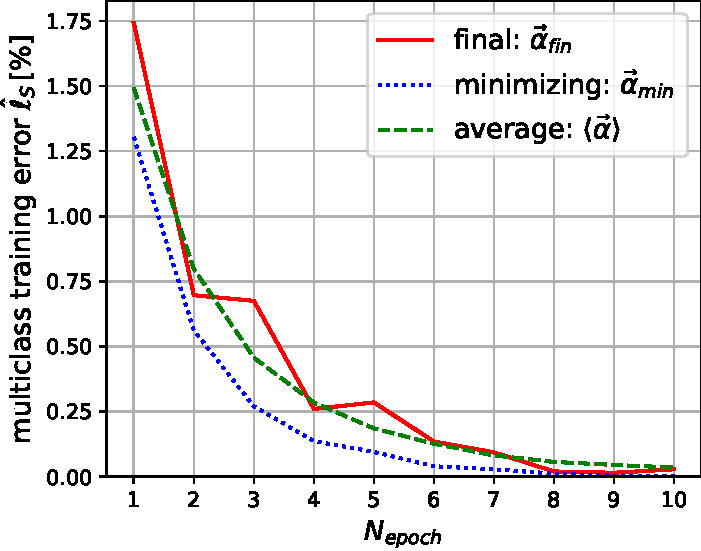
\includegraphics[width=\linewidth]{performance/training_deg=3.pdf} 
        \caption{$p = 3$}
    \end{subfigure}
    \hfill
    \begin{subfigure}[t]{0.49\textwidth}
        \centering
        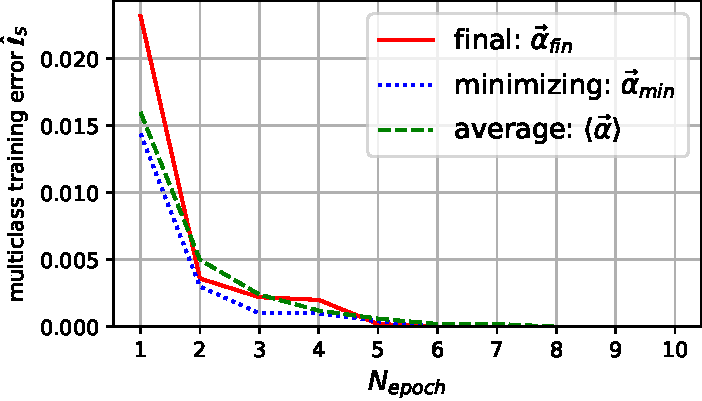
\includegraphics[width=\linewidth]{performance/training_deg=4.pdf} 
        \caption{$p = 4$}
    \end{subfigure}
    \par\bigskip
        \begin{subfigure}[t]{0.49\textwidth}
        \centering
        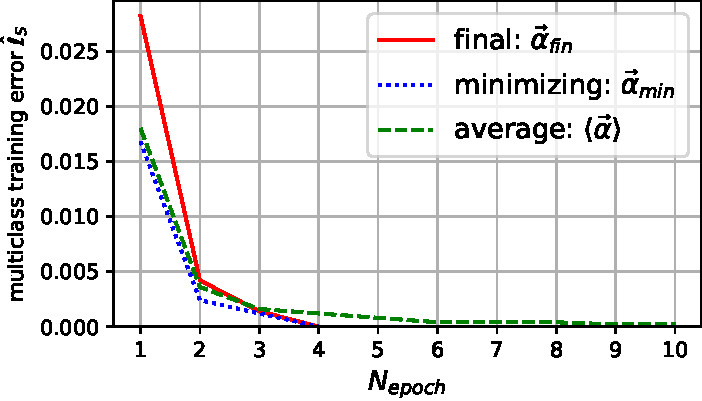
\includegraphics[width=\linewidth]{performance/training_deg=5.pdf} 
        \caption{$p = 5$}
    \end{subfigure}
    \hfill
    \begin{subfigure}[t]{0.49\textwidth}
        \centering
        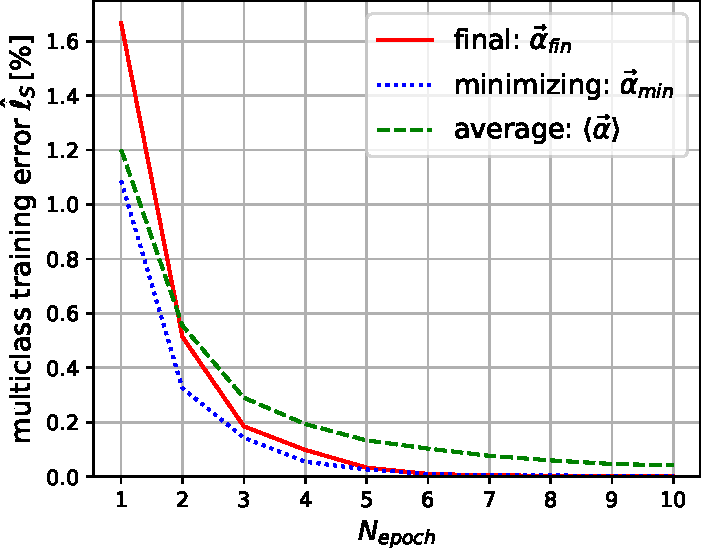
\includegraphics[width=\linewidth]{performance/training_deg=6.pdf} 
        \caption{$p = 6$}
    \end{subfigure}
    \caption{Multiclass training error rates $\hat{\ell}_{S}$ as a function of the number of epochs $N_{epoch}$ for the training of multiclass predictors on the MNIST training set $S$. The multiclass predictors classify given images of handwritten digits with a label between $0$ and $9$. Each panel displays the multiclass training error rates $\hat{\ell}_{S}$ for a different degree $p$ of the polynomial kernel for the three approaches to retrieve binary predictors inside the multiclass kernel perceptron algorithm. Note, the different scales of the vertical axes. The multiclass test error rates for the same multiclass predictors are displayed in Fig~\ref{fig:test_error_multi}.}
    \label{fig:train_error_multi}
\end{figure}

\begin{figure}[h!]
    \begin{subfigure}[t]{0.49\textwidth}
        \centering
        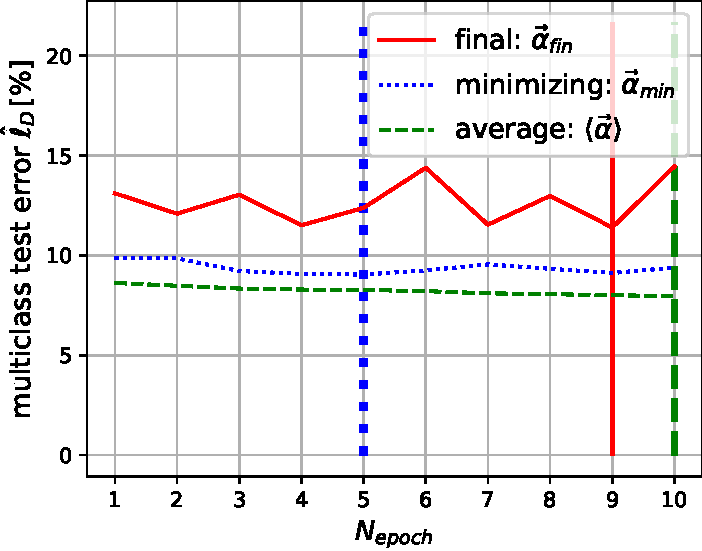
\includegraphics[width=\linewidth]{performance/test_deg=1.pdf} 
        \caption{$p = 1$}
    \end{subfigure}
    \hfill
    \begin{subfigure}[t]{0.49\textwidth}
        \centering
        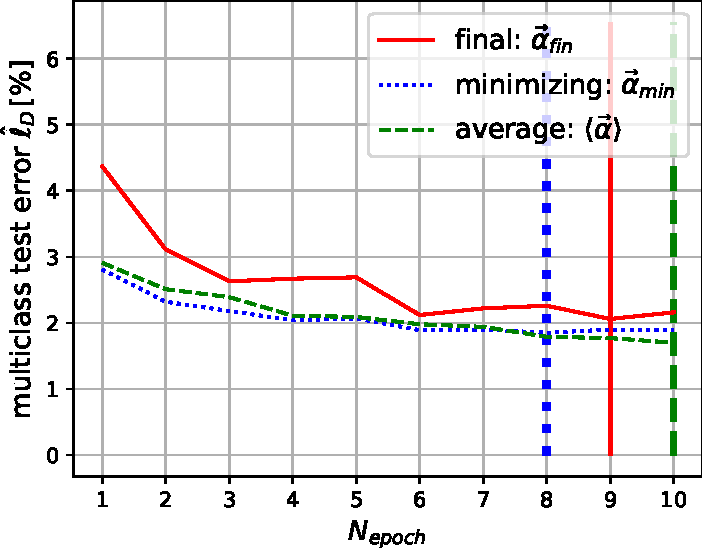
\includegraphics[width=\linewidth]{performance/test_deg=2.pdf} 
        \caption{$p = 2$}
    \end{subfigure}
    \par\bigskip
        \begin{subfigure}[t]{0.49\textwidth}
        \centering
        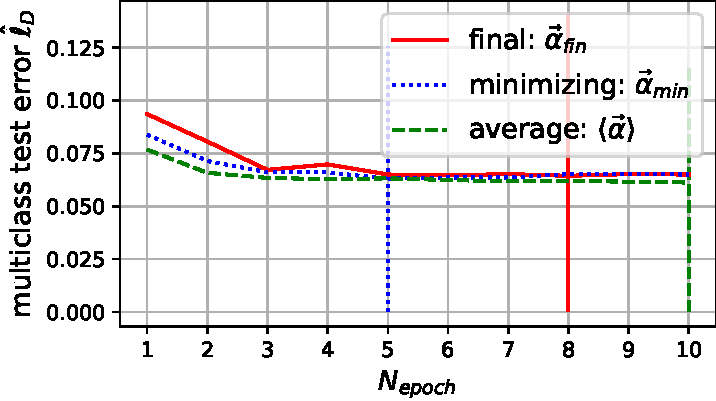
\includegraphics[width=\linewidth]{performance/test_deg=3.pdf} 
        \caption{$p = 3$}
    \end{subfigure}
    \hfill
    \begin{subfigure}[t]{0.49\textwidth}
        \centering
        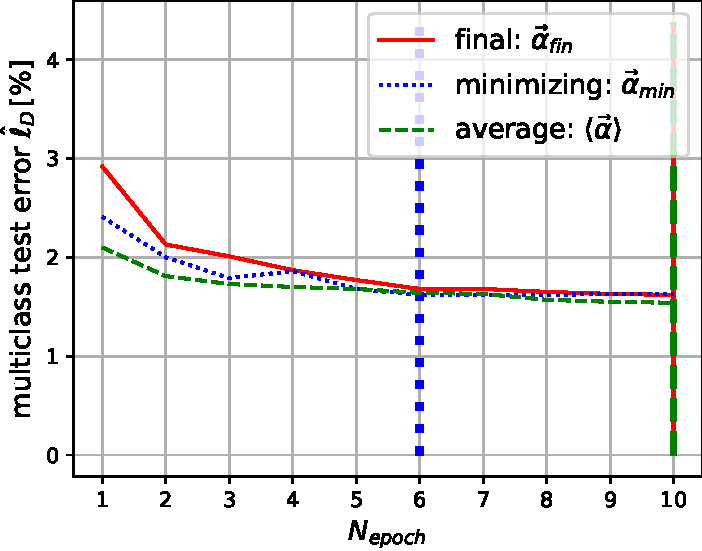
\includegraphics[width=\linewidth]{performance/test_deg=4.pdf} 
        \caption{$p = 4$}
    \end{subfigure}
    \par\bigskip
        \begin{subfigure}[t]{0.49\textwidth}
        \centering
        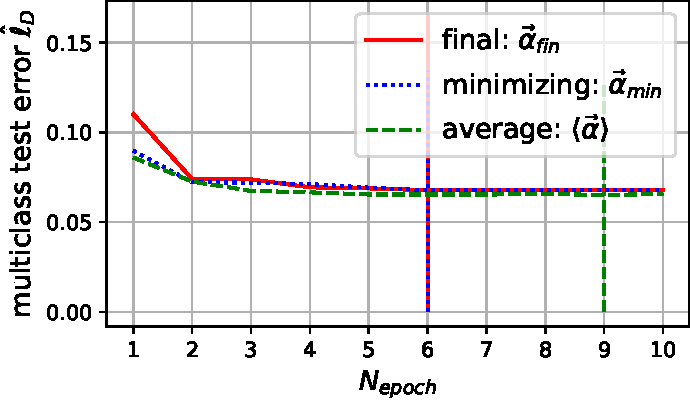
\includegraphics[width=\linewidth]{performance/test_deg=5.pdf} 
        \caption{$p = 5$}
    \end{subfigure}
    \hfill
    \begin{subfigure}[t]{0.49\textwidth}
        \centering
        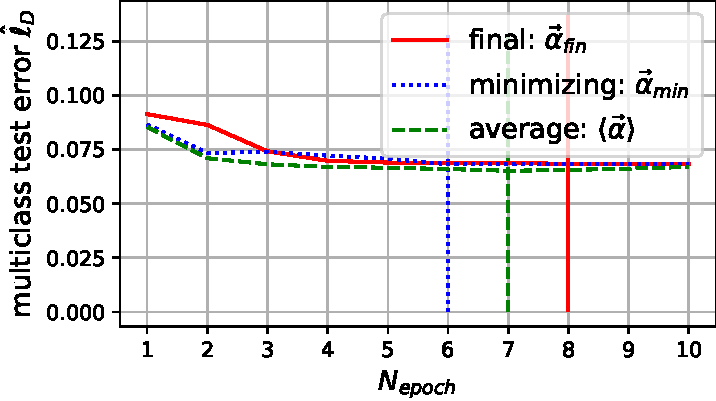
\includegraphics[width=\linewidth]{performance/test_deg=6.pdf} 
        \caption{$p = 6$}
    \end{subfigure}
    \caption{Multiclass test error rates $\hat{\ell}_{D}$ as a function of the number of epochs $N_{epoch}$ for the training of multiclass predictors on the MNIST training set $S$. The multiclass predictors classify given images of handwritten digits with a label between $0$ and $9$. Each panel displays the multiclass test error rates $\hat{\ell}_{D}$ for a different degree $p$ of the polynomial kernel for the three approaches to retrieve binary predictors inside the multiclass kernel perceptron algorithm. Note, the different scales of the vertical axes. The multiclass training error rates for the same multiclass predictors are displayed in Fig~\ref{fig:train_error_multi}. In each panel, the vertical lines indicate the number of epochs $N_{epoch}$ with the smallest test error rate for all three predictor types. The results are also reported in Tab.~\ref{tab:min_test}.}
    \label{fig:test_error_multi}
\end{figure}

\begin{center}
\begin{tabular}{c||c|c|c}
& $\vec{\alpha}_{fin}$ & $\vec{\alpha}_{min}$ & $\langle \vec{\alpha} \rangle$\\
\hline
\hline
$\hat{\ell}_D\,[\%]$ & \boldmath$1.58$ & \boldmath$1.55$ & \boldmath$1.54$\\
$\hat{\ell}_S\,[\%]$ & $0.0150$ & $0.127$ & $0.0200$ \\
$p$ & $3$ & $3$ & $4$\\
$N_{epoch}$ & $9$ & $6$ & $10$
\end{tabular}
\end{center}

\begin{figure}
\centering
	\begin{subfigure}[t]{0.49\textwidth}
	\centering
		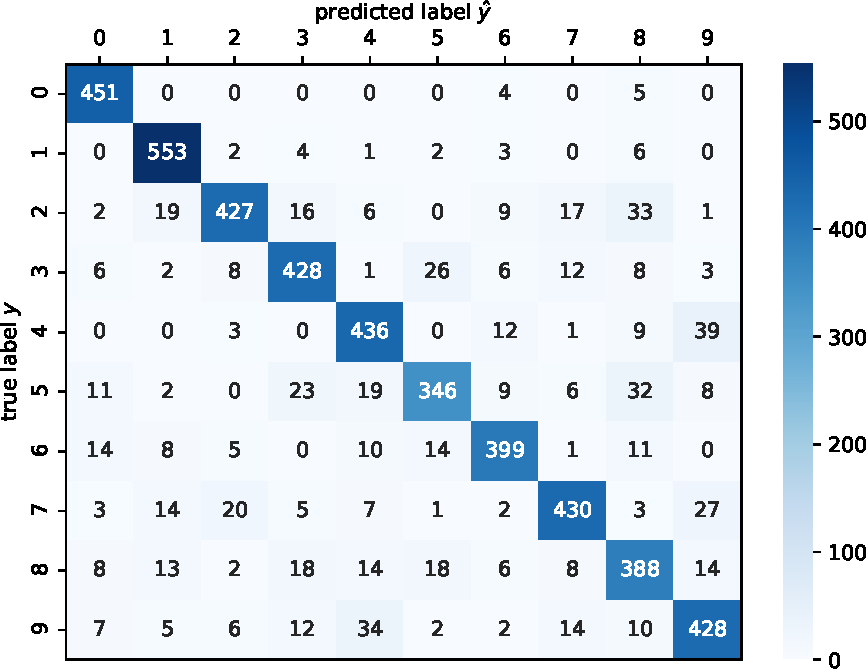
\includegraphics[width=\linewidth]{conf_mat/predictor.pdf} 
		\caption{final predictor $\vec{\alpha}_{fin}$}
	\end{subfigure}
	\hfill
	\begin{subfigure}[t]{0.49\textwidth}
	\centering
		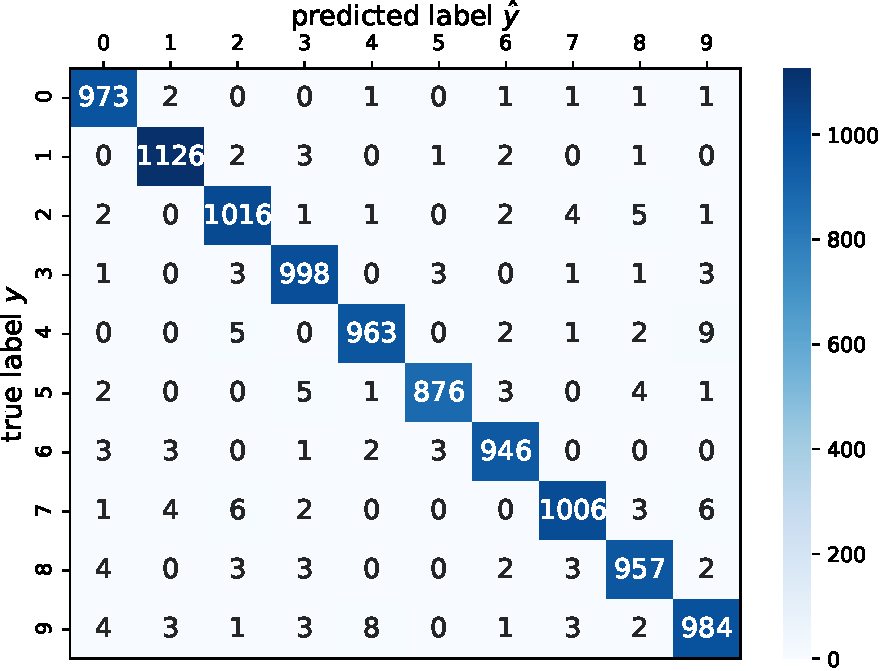
\includegraphics[width=\linewidth]{conf_mat/min_predictor.pdf} 
		\caption{minimizing predictor $\vec{\alpha}_{min}$}
	\end{subfigure}
		\begin{subfigure}[t]{0.49\textwidth}
	\centering
		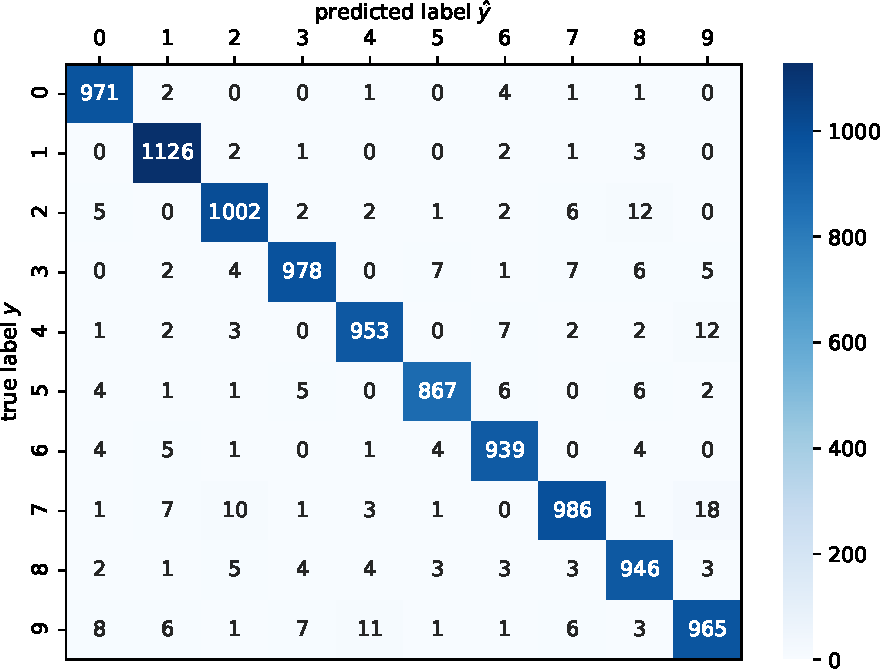
\includegraphics[width=\linewidth]{conf_mat/avg_predictor.pdf} 
		\caption{avearge predictor $\langle\vec{\alpha}\rangle$}
	\end{subfigure}
	\caption{confusion matrix}\label{fig:conf_mat}
\end{figure}

\subsection{Minimizing the Test Error Rate}\label{subsec:best_pred}
